\iffalse
\documentclass[journal,12pt,twocolumn]{article}
\usepackage{graphicx}
\graphicspath{{./figs/}}{}
\usepackage{amsmath,amssymb,amsfonts,amsthm}
\newcommand{\myvec}[1]{\ensuremath{\begin{pmatrix}#1\end{pmatrix}}}
\let\vec\mathbf
\title{
Matrix-Lines
}
\author{SHREYASH CHANDRA PUTTA}
\begin{document}
\maketitle
\tableofcontents

\section{Problem Statement}
\fi
A line perpendicular to the line segement joining the points (1,0) and (2,3) divides it in the ratio $1:n$. Find the equation of the line.
	\begin{figure}[!ht]
		\centering
 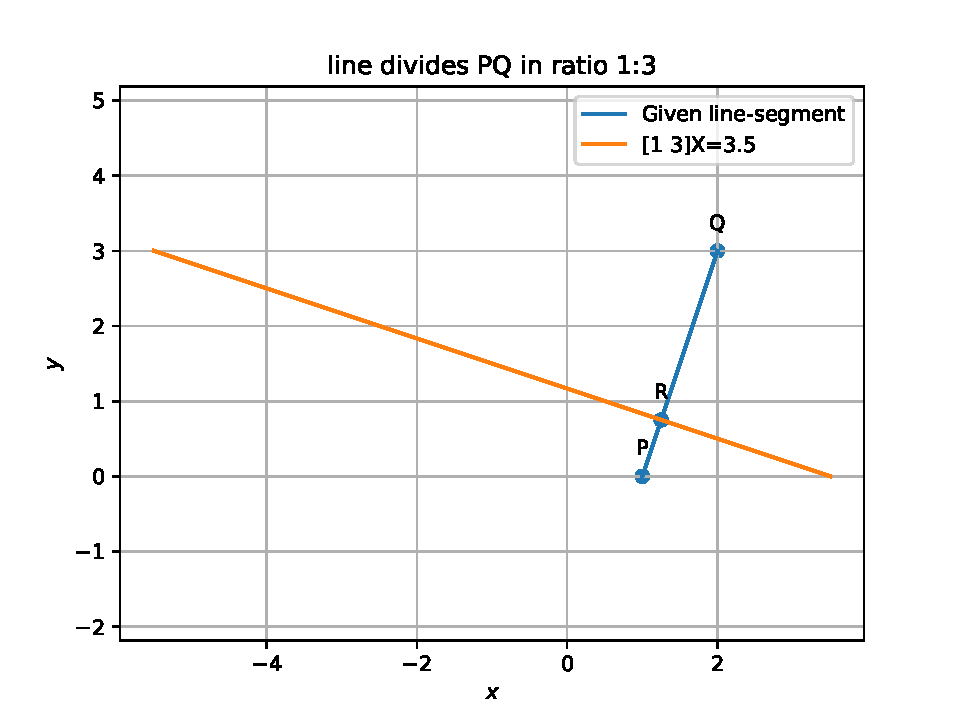
\includegraphics[width=\columnwidth]{chapters/11/10/2/11/figs/linefig.pdf}
		\caption{}
		\label{fig:11/10/2/11}
  	\end{figure}
	\\
	\solution 
\iffalse
(note: we are taking n as user Input) .

% 

\begin{table}[h]
    \centering
    \begin{tabular}{|c|c|c|}
       \hline
       \textbf{Symbol}&\textbf{Value}&\textbf{Description}  \\
       \hline
	    $\vec{P}$ & $\myvec{
		    1\\
		    0}$
	    & given point\\
        \hline
	    $\vec{Q}$ & $\myvec{2\\3}$
 & given point\\
        \hline
	    $\vec{R}$ & $\myvec{
  \frac{2+n}{1+n}\\
  \frac{3}{1+n}}$
 & intersecting point  \\
       \hline
    \end{tabular}
    \caption{Parameters}
    \label{tab:my_label}
\end{table}

%\section{Construction}

\begin{figure}[h]
    \centering
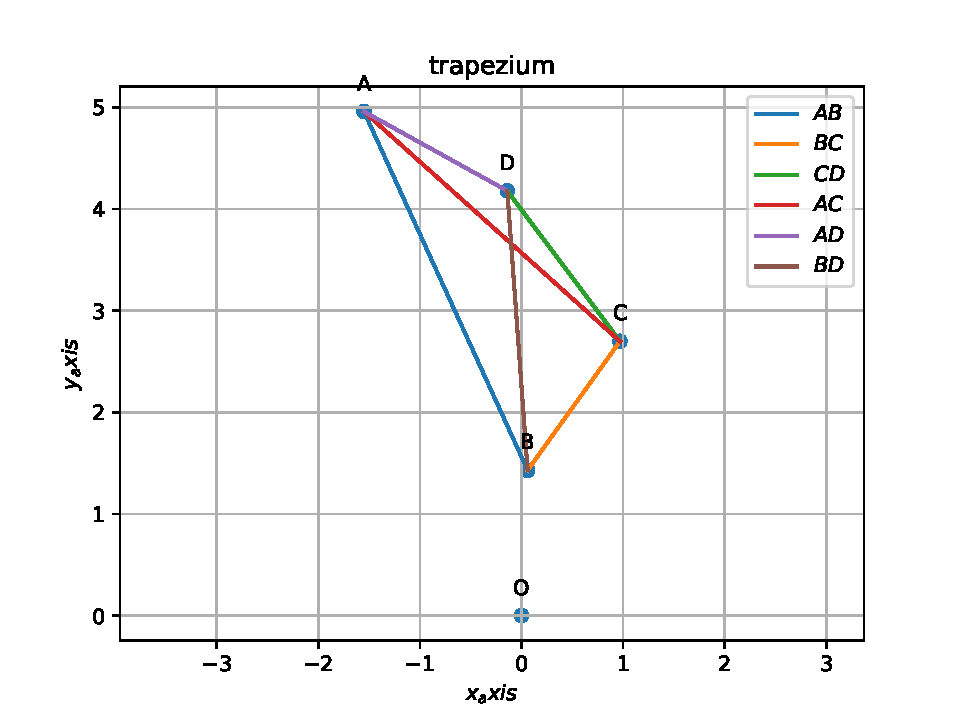
\includegraphics[width=\columnwidth]{fig/linefig.pdf}
    \caption{Equation of the required Straight Line}
    \label{fig:my_label}
\end{figure}




\section{Solution}

Given that resultant will divide the equation of line in the ratio 1:n and the line is perpendicular to line segment joining the points (1,0)and(2,3)  ) \\
%so, b = 9 - a  \\
\\
\fi 
Let 
\begin{align}
{\vec{P}}=\myvec{
  1\\
  0},
 {\vec{Q}}=\myvec{
  2\\
  3}
\end{align}
\iffalse
%	\vec{n^{\top}}
%	\myvec{
 % a\\
  %0}
  %= c \label{eq-1}
%\end{align}
\\
\fi
The direction vector of 
$PQ$ is 
\begin{align}
	\vec{m}=
     \vec{Q
 }-  \vec{P
 }
=
     \myvec{
  1\\
  3
 }
\end{align}
\iffalse
\\
We know, that position or  directional vector of points P and Q line segement used as the normal vector
\\
\\
 The general equation of the required perpendicular line is
 ${\vec{M^{\top}}\vec{X}} = c$.
 \\
 \\
 The perpendicular line cutting a line segment P and Q in ratio 1:n is passes through the point R.
 \fi
 Also, using section formula, 
 \begin{align}
	 \vec{R}=\frac{\vec{Q}+n\vec{P}}{1+n}
\end{align}
and the 
equation of line passing through ${\vec{R}}$ is
\begin{align}
	\vec{m}^{\top}\brak{\vec{x}-\vec{R}}=0
\\
\implies 
	   \myvec{
		   1 &  3}\vec{x}
	   &= \myvec{
  1\ 3}\myvec{
  \frac{2+n}{1+n}\\
  \frac{3}{1+n}} 
  \\
	&=	  \frac{11+n}{1+n} 
\end{align}
\iffalse



 
\section{Software}
Download the following code using,
\begin{table}[h]
    \centering
    \begin{tabular}{|c|}
    \hline \\
         svn co https://github.com/chanduputta/ \\FWC-Module1Assignments/blob/\\main/assignment4/line/lines3.py  \\
         \\
\hline
    \end{tabular}
\end{table}
\\
and execute the code by using command
\begin{center}
	\textbf{cmd:}
{Python3  lines3.py}\\
	\textbf{Then,}
{input your required n value}
\end{center}

\section{Conclusion}
\begin{center}
We found the equation of a line perpendicular to the line segement joining the points (1,0)and(2,3) divides it in the ratio 1:n .
\end{center}
\end{document}
\fi
